% !TEX root = ./main.tex
\section{GraphCoQL}\label{sec:form}

\fo{Review this after all} In this section we describe our formalization of GraphQL in Coq. We start by defining a schema and its properties, then the graph data model and finally we review queries and their semantics. The definitions are as close as possible with respect to the \spec{}. This eyeball correspondence between the english-written definitions and the code gives a first level of trust that our formalization is correct, following the examples of X, Y and Z. Whenever there is a mismatch we point it out and explain the reasoning behind each decision.


\subsection{GraphQL Schema}\label{subsec:schema}
We formalize schemas and type definitions following the \spec{}. A schema is represented as a record, containing a list of type definitions and a root type that specifies the available queries (\eg \texttt{Query} in the example from Figure \ref{fig:schema_ex}):
%

\begin{minted}[bgcolor=coqbg]{coq}
Record graphQLSchema := GraphQLSchema {
    query_type : Name;
    type_definitions : seq TypeDefinition }.
\end{minted}
%
Schemas may also include additional root types for specifying mutations and subscriptions\footnote{https://graphql.github.io/graphql-spec/June2018/\#sec-Schema}. These operations are, however, out of the scope of our formalization.

Our formalization of type definitions closely follows the \spec, as depicted in Figure~ \ref{fig:types_def}. A type may be a scalar type, an object type, which possibly implements a set of interfaces, an interface type, a union type or an enumeration type. Object and interface type definitions comprise an (ordered) set of fields; union types are defined by a set of type names and enumeration types by a set of values. For the corresponding type definitions to be valid, all such three sets should not be empty. While the \spec enforces this requirement syntactically (see the grammar on the left of Figure~ \ref{fig:types_def}), we perform this validation when verifying the (overall) well-formedness schemas.     
%
\setlength{\grammarparsep}{10pt plus 1pt minus 1pt} % increase separation between rules
\begin{figure*}[h]
    \centering
    \begin{subfigure}{.5\textwidth}
    \begin{grammar}
    <TypeDefinition> ::= \textbf{\texttt{scalar}} <name>
%    \alt \textbf{\texttt{type}} <name> \textbf{\texttt{\{}} <Field>$^{+}$ \textbf{\texttt{\}}}
    \alt \textbf{\texttt{type}} <name> [\textbf{\texttt{implements}} <name>$^{+}$] \textbf{\texttt{\{}} <Field>$^{+}$ \textbf{\texttt{\}}}
    \alt \textbf{\texttt{interface}} <name> \textbf{\texttt{\{}} <Field>$^{+}$ \textbf{\texttt{\}}}
    \alt \textbf{\texttt{union}} <name> \textbf{\texttt{=}} <name> (\textbf{\texttt{|}} <name>)*
    \alt \textbf{\texttt{enum}} <name>  \textbf{\texttt{\{}}  <name>$^{+}$ \textbf{\texttt{\}}}

    <Field> ::= <name> \textbf{\texttt{(}} <Arg>* \textbf{\texttt{) :}} <type>

    <Arg> ::= <name> \textbf{\texttt{:}} <type>

    <type> ::= <name>
    \alt \textbf{\texttt{[}}  <type> \textbf{\texttt{]}}
    \end{grammar}

    \end{subfigure}%
    \begin{subfigure}{.5\textwidth}
    \begin{minted}[bgcolor=coqbg]{coq}
    Inductive TypeDefinition : Type :=
    | ScalarTypeDefinition (name : Name)
    | ObjectTypeDefinition (name : Name)
                           (interfaces : seq Name)
                           (fields : seq FieldDefinition)
    | InterfaceTypeDefinition (name : Name)
                              (fields : seq FieldDefinition)
    | UnionTypeDefinition (name : Name)
                          (members : seq Name)
    | EnumTypeDefinition (name : Name)
                         (members : seq EnumValue).

    Inductive type : Type :=
    | NamedType : Name -> type
    | ListType : type -> type.
    \end{minted}

    \end{subfigure}
    \caption{Definition of GraphQL types, the \spec{}'s grammar (left) and Coq implementation (right). Square brackets represent optional values. \fo{In the grammar, I would push the scalar case to a new line, to match the Coq snippet on the right}}
    \label{fig:types_def}
\end{figure*}


% As can be seen from the figure, our implementation looses information about non-emptiness of fields, union and enum members. We push this validation to a posterior predicate, as well as the discussion about the reasons behind this decision, to the following paragraphs.

% As can be seen in the figure, we tried to match the \spec{}'s definition as much as possible. This eyeball correspondence gives us a degree of confidence about the implementation.  % We currently do not include the \textit{Input Object} types, as well as anything related to \textit{introspection}.

On this regard, observe that the provided definitions of schema and types enable building ``invalid'' schemas. For instance, one can build an object that implements scalar types or use a nonexistent type as the query type. To avoid this problem, the \spec provides several validation rules, scattered throughout the document\footnote{Most can be found in the \textbf{Type Validation} subsection of each type described in https://graphql.github.io/graphql-spec/draft/\#sec-Type-System.}.  We collect these rules and refer to them as the \textit{well-formedness} condition of a GraphQL schema.


\begin{definition}
A GraphQL schema is \textit{well-formed} if: 
\begin{itemize}
    \item its root type (is defined and) is an object type, 
    \item there are no duplicated type names, and
    \item every type definition is \textit{well-formed}.
\end{itemize}
\end{definition}

In our Coq formalization, this is captured by the Boolean predicate below. As mentioned in the introduction, our formalization heavily relies on Boolean reflection, following the SSReflect mindset.
%
\begin{minted}[bgcolor=coqbg]{coq}
Definition is_a_wf_schema (s : graphQLSchema) : bool :=
      is_object_type s s.(query_type) &&
      uniq s.(schema_names) &&
      all is_wf_type_def s.(type_definitions).
\end{minted}
%
The notion of well-formedness for type definitions requires \eg that union members contain existent object types and that object and interface types contain at least one field. Due to space limitations, we omit the full definition and refer the interested reader to file \texttt{SchemaWellFormedness.v}.

%We will, though, resume the discussion about non-emptiness of fields, union and enum members, which are included in the predicate. The main reason behind this decision is that, even though the \spec{} embeds this information in the grammar, it still includes it in their validation rules later on. We believe that it is simpler to use common lists instead of defining new structures or using dependent types, from an implementation point of view, while still preserving the correspondence to the algorithmic description given by the \spec{}.
%\td{Not sure if correctly worded... but it was just simpler to use lists. A non-empty list structure required coercions to lists and then redefining some lemmas and things. Or using dependent types (sigma type) adds complexity when proving and defining things (at least that was the case for me)}


% There are two main reasons why we push this rule to a separate predicate instead of embedding it in the structure itself. The first one is that, even though the \spec{} embeds it in the grammar, it still includes it in a validation rule later on. To match their definition and preserve the eyeball correspondence, we also include it. The second reason is that we use SSReflect and it is simpler to use \mintinline{coq}{seq} directly and all its theory, instead of defining coercions and repeating definitions for a new structure.

For convenience, we encapsulate schemas with their well-formedness proof in a single structure. This structure also contains predicate \mintinline{coq}{is_a_valid_value}, which determines whether a value used in a query indeed matches the scalar type expected by the schema. For example, if a field argument has type \texttt{Float}, the \spec requires that the actual argument used in query represent a double-precision fractional value.\footnote{The \spec{} declares a set of minimal scalar values and how they should be represented, such as floating-point values adhering to IEEE 754. We do not include this base restrictions but leave it open to implementation.}
%
\begin{minted}[bgcolor=coqbg]{coq}
Record wfGraphQLSchema := WFGraphQLSchema {
    schema : graphQLSchema;
    _ : schema.(is_a_wf_schema);
    is_a_valid_value : type -> Vals -> bool; }.
\end{minted}

% This predicate is necessary to establish when a value used in a query or in the graph actually matches the scalar type expected by the schema. For instance, if an argument requires a \texttt{Float} value, then the actual value passed to the query must be something that represents a double-precision fractional value\footnote{The \spec{} declares a set of minimal scalar values and how they should be represented, such as floating-point values adhering to IEEE 754. We do not include this base restrictions but leave it open to implementation.}. This predicate validates that this is satisfied.

% Due to space constraints, we omit the definition of \textit{well-formedness} for type definitions. This property includes things such as: interfaces and objects must declare at least one field, objects correctly implement their declared interfaces, union types are not empty and contain only object types, amongst others. These definitions are collected from the \spec{} \td{Scattered throughout the \spec{}*}.

Having reviewed or formalization of schemas, we now discuss our formalization of the data model. 


\iffalse
\begin{minted}{coq}
Let Animal := Interface "Animal" {[::
                (Schema.Field "name" [::] "String");
                (Schema.Field "friends" [::] ["Animal"])
            ]}.
Let Dog := Object "Dog" implements [:: "Animal"] {[::
            (Schema.Field "name" [::] "String");
            (Schema.Field "friends" [::] ["Animal"]);
            (Schema.Field "favouriteToy" [::] "Toy")
        ]}.
\end{minted}
\fi


\subsection{GraphQL Data model}\label{subsec:graph}
Following \HP, for our formalization we adopt a data model based on graph, where data are modeled as directed property graphs, with labeled edges and typed nodes. Nodes contain a type and a set of properties (key-value pairs) and  edges contain single labels that describe the relation between nodes. Also, every property and label may contain a list of arguments (key-value pairs).

To represent the values associated to properties or arguments, we consider the type \Vals. A value in \Vals may be a single scalar value or a list of values\td{This choice is based on the limitations of the model}.\fo{I think we should address this in the Discussion section, where we discuss the limitations of our formalization. We could even remove the last sentence from the paragraph.}

\begin{definition}
A \emph{GraphQL graph} over \Vals{} is defined by the following elements:
\begin{itemize}
    \item A root node.
    \item A collection of edges of the form ($u$, \texttt{f[}$\alpha$\texttt{]}, $v$), where $u, v$ are nodes and \texttt{f[}$\alpha$\texttt{]} is a label with arguments (key-value pairs).
\end{itemize}
\end{definition}

In our formalization, this is captured by the following structures, where \texttt{fld} represents labels over an edge or keys in a node's property. \td{Probably the name is not the best}\fo{Fully agree. I suggest changing \texttt{fld} to \texttt{label}, \texttt{Field} to \texttt{Label} and \texttt{label} to \texttt{name} (or \texttt{lname} if there is a clash) }. 
%
\begin{minted}[bgcolor=coqbg]{coq}
Record fld := 
Field { label : string; args : seq (string * Vals) }.

Record node := 
Node { ntype : Name; nprops : seq (fld * Vals) }.

Record graphQLGraph := 
  GraphQLGraph { root : node; E : seq (node * fld * node) }.
\end{minted}
%
\fo{Tomás, why did you represent graphs as a seq---rather than as a set--of edges?} The root node of a GraphQL graph represents the starting point from where queries are evaluated.

Intuitively, the data modeled by a GraphQL graph is expected to follow (the type system described by) a schema. However, the definition of graphs is fully independent schemas. To relate the data to the type system, we define the notion of \textit{conformance} of a graph \wrt a schema.
%
\begin{definition}
A GraphQL graph $g$ \textit{conforms} to a schema $s$ if:
\begin{itemize}
    \item the types of $g$ root node and $s$ query root coincide, 
    \item every edge of $g$ \textit{conforms} to $s$, and
    \item every node of $g$ \textit{conforms} to $s$.
\end{itemize}
\end{definition}
%
The conformance of nodes includes rules such as checking that a node type is declared as an object type in the schema and that its properties are defined as fields in the corresponding type. Among others, the conformance of edges ensures that edge labels are declared as a field in the source node's type and the target node has a type compatible with the field's return type. Full definitions of these two notions are found in file \texttt{GraphConformance.v}.

With this in mind, the notion of conformance of a graph \wrt a schema is formalized as follows:
%
\begin{minted}[bgcolor=coqbg]{coq}
Definition is_a_conforming_graph 
      (s : wfGraphQLSchema) (g : graphQLGraph) : bool :=
  root_type_conforms s g.(root) &&
  edges_conform s g &&
  nodes_conform s g.(nodes).
\end{minted}
%
As a side note, this notion was only loosely defined in \HP, but it is properly addressed in a recent work of one of its authors ~\cite{olafschema}.

Similarly to GraphQL schemas, we define a structure that encapsulates the notion of a \textit{conformed} graph, containing a graph and a proof of its conformance to a particular schema.

\begin{minted}[bgcolor=coqbg]{coq}
Record conformedGraph (s : wfGraphQLSchema) :=
  ConformedGraph { graph : graphQLGraph;
                       _ : is_a_conforming_graph s graph }.
\end{minted}

 %These properties include validation rules such as: every node must have an object type and their properties must be defined in their associated type, or an edge's label must be declared as a field in the source node's type and the target node must have a type compatible to the field's return type, among other things.

%With both the schema and the underlying data model we can proceed to define GraphQL queries and their semantics.


\subsection{GraphQL Query}\label{subsec:query}
To define queries we faithfully follow the \spec, as shown in Figure~\ref{fig:query_def}. A query can be a single field, a field followed by a set of subqueries or an inline fragment comprising a type condition and a set of subqueries. Field can be accompanied by a list of arguments and can also be renamed.

\begin{figure*}[h]
  \centering
  \begin{subfigure}{.5\textwidth}
    \begin{grammar}
        <Query> ::= <name> \textbf{\texttt{(}} <Arg>* \textbf{\texttt{)}}
        \alt <alias> \textbf{\texttt{:}} <name> \textbf{\texttt{(}} <Arg>* \textbf{\texttt{)}}
        \alt <name> \textbf{(} <Arg>* \textbf{)} \textbf{\texttt{\{}} <Query>$^{+}$ \textbf{\texttt{\}}}
        \alt <alias> \textbf{\texttt{:}} <name> \textbf{\texttt{(}} <Arg>* \textbf{\texttt{)}} \textbf{\texttt{\{}} <Query>$^{+}$ \textbf{\texttt{\}}}
        \alt \textbf{\texttt{... on}} <name> \textbf{\texttt{\{}} <Query>$^{+}$ \textbf{\texttt{\}}}
        
        <Arg> ::= <name> \textbf{\texttt{:}} <value>
    \end{grammar}
  \end{subfigure}%
  \begin{subfigure}{.5\textwidth}

    \begin{minted}[bgcolor=coqbg]{coq}
    Inductive Query : Type :=
    | SingleField (name : Name)
                  (arguments : seq (Name * Vals))
    | AliasedField (alias : Name)
                   (name : Name)
                   (arguments : seq (Name * Vals))
    | NestedField (name : Name)
                  (arguments : seq (Name * Vals))
                  (subqueries : seq Query)
    | NestedAliasedField (alias : Name)
                         (name : Name)
                         (arguments : seq (Name * Vals))
                         (subqueries : seq Query)
    | InlineFragment (type_condition : Name)
                     (subqueries : seq Query).
    \end{minted}
  \end{subfigure}
  \caption{Definition of GraphQL queries, the \spec{}'s grammar (left) and the Coq implementation (right).\fo{To be consistent with what you do for \texttt{NestedField}, rename \texttt{AliasedField} to \texttt{SignleAliasedField}. Also, in the grammar, push the first constructor to a new line, to match the way you display it in the Coq formalization on the right}}
  \label{fig:query_def}
\end{figure*}

Intuitively, a valid query will have a tree structure, where leaves correspond to fields of scalar types and inner nodes correspond either to fields of some object type or abstract type \fo{abstract type not defined}, or to inline fragments that condition when their subqueries are evaluated. 

\iffalse
%For instance, the query in Figure \ref{fig:qres_ex} can be depicted as the tree in Figure \ref{fig:query_tree}.
\begin{figure}
    \centering
    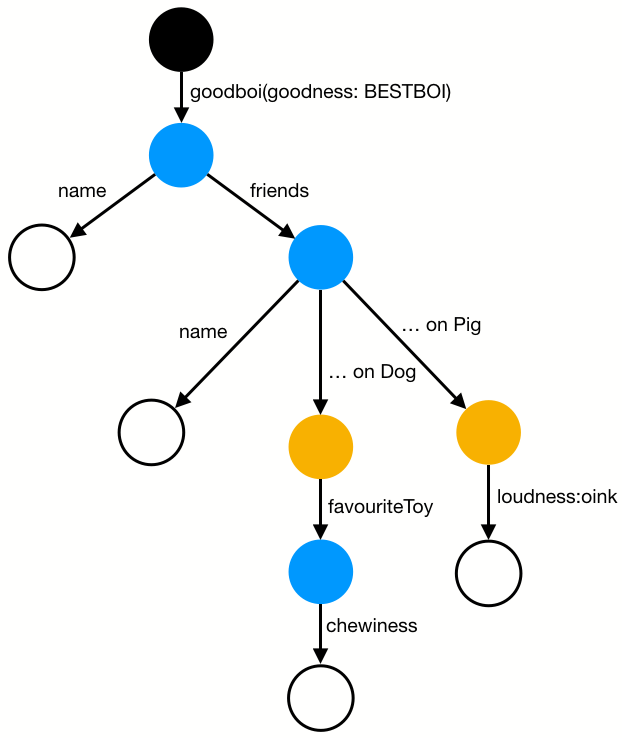
\includegraphics[scale=0.33]{imgs/query_tree.png}
    \caption{GraphQL query as a tree.}
    \label{fig:query_tree}
\end{figure}
\fi 

% Similar to the schema definition, we follow the \spec{}'s grammar as closely as possible, as can be seen from Figure~\ref{fig:query_def}. We do not embed the property of non-emptiness of subqueries in the definition because the \spec{} pushes it to a different validation rule, even though it is already embedded in the grammar, and we believe it is simpler to reuse the \texttt{seq} library and its existent functionalities. 

Observe that the definition of queries in Figure~\ref{fig:query_def} is not bound to any schema, requiring thus a separate validation process to ensure that they respect or adhere to a given schema. We introduce the notion of query \textit{conformance}, based on a set of validation rules scattered throughout the \textit{Validation} section of the \spec{}\footnote{https://graphql.github.io/graphql-spec/June2018/\#sec-Validation}. The validity of queries depends on a notion of \textit{type in context} at a given query location.\footnote{The \spec refers to it as type in scope or parent type. Some algorithmic descriptions make use of the types in context but are not explicit in their signatures.} % Since queries are selections over the fields of types, it is important to know exactly to what type they are being applied.
To illustrate this, consider the following query with two occurrences of field \texttt{name}.

%\begin{minipage}[t]{.25\textwidth}
\begin{minted}[escapeinside=||, mathescape=true]{js}
query {
  goodboi {
    |$\ldots$| on Dog {
      name
      favoriteToy
    }
    |$\ldots$| on Pig {
      name
      favoriteToy
    } } }
\end{minted}
%\end{minipage}%
% \begin{minipage}[t]{.25\textwidth}
% \begin{minted}[escapeinside=||, mathescape=true]{js}   
% type Human {
%   age: Int
% }

% type Martian {
%   age: Float
% }
% \end{minted}
% \end{minipage}
\et{for space reason, we may want to take some liberties wrt the formatting of queries and responses (see some examples on this page)}


\noindent In one case, the field is requesting information about the \texttt{Dog} type, while in the other it is requesting information about case about the \texttt{Pig} type. (These are the respective types in context for the first and second occurrence of the field.) The distinction is important because some field selections might be valid in some contexts but not in others. This is the case, for instance, for field \texttt{favoriteToy}: It is valid in the context of a \texttt{Dog} type but it is invalid in the context of a \texttt{Pig} type, as \texttt{Pig} type does not contain any such field. Similarly, the above query would also be invalid if \texttt{Pig} type contained a so-called field, but of type different from \texttt{Toy} ---the type the same field in type \texttt{Dog}.

%Just as in the case of well-formedness of schemas or conformance of graphs, queries must go through a validation process. We define the property of \textit{conformance} of queries, based on validation rules scattered throughout the \textit{Validation} section of the \spec{}\footnote{https://graphql.github.io/graphql-spec/June2018/\#sec-Validation}.

% Before describing the validation process, it is very important to address the notion of \textit{type in context} where queries are defined and used. The type in context is the type over which a user might be requesting information on its fields. To illustrate this, consider the following query. The first selection, namely \texttt{goodboi}, is requesting information about the query type, meaning that it is used in the context of the \texttt{Query} type. Moving onto the  \texttt{name} subselection, it is not direct which is. In one case, the type in context is \texttt{Dog}, while in the other the field is used in the context of the \texttt{Pig} type.

% The importance of this type in context is that fields or inline fragments might be valid in certain cases but not in others. Similarly, a field may have a particular return type in one case and a different one in another type, like in the following example. Both types have an \texttt{age} field, but in one case it returns an integer value while in the other a floating point value. If that field is encountered in a query, it is necessary to know to which type it is being requested.

Now that we have clarified the notion of type in context, we are in condition of defining the notion of query conformance. 

\begin{definition}
A GraphQL query $\varphi$ \textit{conforms} to a schema $s$ if:
\begin{itemize}
    \item selections in $\varphi$ are consistent, 

    \item field merging between fields is possible, and
    % During the evaluation process, fields with the same response name are collected and merged to ensure that they are all executed at the same time. This validation rule checks that it makes sense to merge those fields. The following example illustrates two queries that have the same response name but should not be merged. The first one is accessing the field \texttt{name} while the second is accessing the field \texttt{age} but renaming it to \texttt{name}. Both are selections on different fields of the same type but with the same response name.
    % \begin{minted}{graphql}
    %                query {
    %                    name
    %                    name:age
    %                }
    %\end{minted}

    \item fields with same response name have compatible response shapes.\fo{We should be more precise about what we mean by ``shape''}
    % This checks whether two fields with the same response name will produce response values that are consistent to each other. These values should be unambiguous for a user. For instance, the following example\td{These examples look a bit off I think.} shows two queries that produce similar responses but with ambiguous values. In the first one, we ask for dog's \texttt{name}s, which are strings, and in the second for pig's \texttt{age}s, which are integers. We also rename the \texttt{age} value to \texttt{name}. The responses we get will have some cases where \texttt{name} is associated to a string and other where it is associated to integers.
    % \begin{minted}[escapeinside=||,mathescape=true]{graphql}
    %                query {
    %                    |$\ldots$| on Dog {
    %                        name
    %                    }
    %                    |$\ldots$| on Pig {
    %                        name:age
    %                    }
    %                }
    % \end{minted}
\end{itemize}
\end{definition}

In our formalization, this is captured as follows:

%The implementation can be seen in the code below, however due to space limitations we only informally describe the %three mentioned rules. The complete definitions can be found in the file \texttt{QueryConformance.v}.

\begin{minted}[bgcolor=coqbg]{coq}
Definition queries_conform (type_in_scope : Name)
                           (queries : seq Query) : bool :=
        all (is_consistent type_in_scope) queries &&
        is_field_merging_possible type_in_scope queries &&
        have_compatible_response_shapes
            [seq (type_in_scope, q) | q <- queries].
\end{minted}
\fo{This introduces the conformance of a query \wrt a schema, but the schema is never mentioned in the definition. It needs to be fixed!!!}

The first rule specifies when a selection \fo{explain what we mean by a selection} holds by itself. For instance, if the selection is over a field, the rule checks that the field is part of the type in context and that its arguments are provided; if the selection is an inline fragment, then the type condition has to be valid with respect to the type in context \fo{when can it not be valid?}.%The \spec{} defines this rule in several different sections.

The second rule validates when fields can be correctly merged during evaluation, which is an essential aspect of the semantics, since it ensures that repeated fields are only evaluated once. To illustrate this, consider the following query, where a user requests information on the fields \texttt{name} and \texttt{oink} of pigs. The user decides to rename the field \texttt{oink} to \texttt{name}, however this is invalid, since both fields cannot be merged and evaluated once; both fields refer to distinct pieces of information in the system.

\begin{minted}[escapeinside=||,mathescape=true]{js}
query {
  goodboi {
    |$\ldots$| on Pig {
	  name
	  name:oink
} } }
\end{minted}

The last rule is necessary to check when fields generate unambiguous outputs when evaluated. For instance, in the query below a user might request the names of dogs and the oinkness of pigs, but renaming the latter to have the same response name as the former. This query is considered invalid because evaluating it might produce a response that contains entries where the key \texttt{name} is associated to both string values and floating point numbers. 

\begin{minipage}[t]{.22\textwidth}
\begin{minted}[escapeinside=||,mathescape=true]{js}
query {
  goodboi {
    friends {
      |$\ldots$| on Dog {
        name
      }
      |$\ldots$| on Pig {
        name:oink
} } } }
\end{minted}
\end{minipage}%
\begin{minipage}[t]{.22\textwidth}
\begin{minted}[escapeinside=||,mathescape=true]{js}
// Possible invalid output
{
  "goodboi" : {
    "friends" : [
        { "name" : "Marle" },
        { "name" : 9000 }
    ]
}  }
\end{minted}
\end{minipage}



				
These last two rules, for merging and unambiguous values, are defined as a single validation rule in the \spec{}\footnote{https://graphql.github.io/graphql-spec/June2018/\#sec-Field-Selection-Merging}, however we decide to separate them. The first reason, which we cover more extensively in \S\ref{sec:discussion}, is that it is possible to optimize the algorithm by reducing redundant recursive calls. Secondly, splitting facilitates reasoning about the predicates.

% The main issue is that the \spec{} allows for what we call \textit{invalid fragments}, originally described in an issue in the \spec{}'s repository\footnote{https://github.com/graphql/graphql-spec/issues/367}. In a nutshell, the \spec{} allows using fragments with type conditions that can span to multiple unrelated types. These end up not being evaluated due to posterior checks\footnote{https://graphql.github.io/graphql-spec/June2018/\#DoesFragmentTypeApply()}.


This concludes the definition of GraphQL queries and the validation process. \td{Examples can be found in the files \texttt{SpecExamples.v} and \texttt{HPExample.v}}. For the rest of the paper, it is assumed that queries conform to a given schema. 

\subsection{Semantics}\label{subsec:semantics}
Now we have all the prerequisites to define the semantics of GraphQL queries. We begin by briefly examining the responses generated by executing queries and then we give an informal description of the semantics, finishing with the formal definition. %We finish by discussing some implementation choices and comparison with the \spec{} and \HP{}.

A first observation we need to make is that query semantics is not compositional, in the sense that the result of a sequence of queries is not obtained by concatenating the results of the individual queries. Therefore, our semantic function will take a (whole) sequence of queries and return a (whole) sequence of responses.  

We model individual responses with a tree structure, similar to JSON, as shown below:
%
\begin{minted}[bgcolor=coqbg]{coq}
Inductive Response  : Type :=
| BaseResponse : option Vals -> ResponseNode
| ObjectResponse : seq (Name * ResponseNode) -> ResponseNode
| ArrayResponse : seq ResponseNode -> ResponseNode.
\end{minted}
\fo{I renamed the type name and all the constructors; it was also a polymorphic data structure; I fixed it to \texttt{Option Vals}. Reflect this in the Coq development}

\fo{What is the role of \texttt{ArrayResponse}? When presenting our domain of values \textit{Vals} you mentioned that it can be a scalar value, or a ``list'' of values. Is the \texttt{ArrayResponse} the counterpart of this ``list''? }

\fo{Explain the role of each constructor}
\fo{Shouldn't the ObjectResponse constructor take a GraphQLResponse argument?}

Our treatment of query responses differs from that in the \spec, where responses are just maps \fo{from what to what}
as depicted in Figure~\ref{fig:responses}. We choose this structure to preserve similarity to queries and because it provides a strong reasoning principle, as well as being simpler to preserve order of the responses. This differs slightly from the \spec{}, which only states that responses are a map and does not impose an ordering of responses, although encourages it\footnote{https://graphql.github.io/graphql-spec/June2018/\#sec-Serialized-Map-Ordering}. We believe that preserving the order is one of the strong selling points for GraphQL (queries and their responses are very similar and easy to read). 

%\begin{figure}[h]
\begin{minted}[bgcolor=coqbg]{coq}
Inductive ResponseNode (A : Type) : Type :=
| Leaf : A -> ResponseNode
| Object : seq (Name * ResponseNode) -> ResponseNode
| Array : seq ResponseNode -> ResponseNode.

Definition GraphQLResponse (Vals: eqType) :=
    seq (Name * (@ResponseNode (option Vals))).
\end{minted}
%\caption{Implementation in Coq of GraphQL responses.}
%\label{fig:responses}
%\end{figure}

\td{Move to discussion?} Our approach has two main disadvantages: possible duplication of response names and cost of access. Since we use lists instead of maps, we can encounter duplicated names and accessing a value has a linear cost given by the lists size, instead of the constant access obtainable with a map. We still argue that the reasoning principles and simplicity to order is highly valuable. Nevertheless, we include a proof that the results obtained with the semantics have no duplicated names. Finally, we use option types to represent null values in the leaves of the response tree.



As we described in \S\ref{subsec:graph}, the underlying data model we use is a graph, therefore the semantics are instantiated to this setting. %In a following paragraph we briefly explore an alternative that is closer to the \spec{}, in the sense that it can be detached from a particular data model. 
Informally, the evaluation of a query then represents a navigation over a graph. At top level, a query begins from the root node and then navigates around its edges and nodes, collecting data along the way. In this sense:
\begin{itemize}
    \item A field selection represents either accessing a node's property or traversing an edge to a neighboring node.
    \item An inline fragment conditions whether using a node to access its properties or to traverse to other nodes.
    \item Subqueries are evaluated in neighboring nodes.
\end{itemize}

The formal definition of the semantics is depicted in Figure \ref{fig:semantics}. The definition displays the cases where a field selection is accessing a node's property, when it is navigating to other nodes and when it is evaluating an inline fragment. Aliased fields are omitted for brevity but the complete definition can be explored in the file \texttt{QuerySemantics.v}.

\td{Move to discussion?}
The main difference with respect to \HP{} and the main similarity to the \spec{} is that we perform a collection of fields at the query level, whereas \HP{} performs a post-processing of responses. The main reasons are our approach is more similar to the \spec{} and that it is harder to reason using \HP{}'s approach.

\td{Don't know how to present this or if it is relevant but I include it so you know it exists - The spec first groups fields by name and then evaluates each group. These are different steps. We define everything in one place because it was easier to reason about the semantics. The difficulty with the spec's approach is that when proving things about the semantics, you have to provide, at each step, the information on how your data is structured (every group contains only fields and every field in a group has the same response name as the group's key used to group them). This is problematic mostly because of inline fragments, which do not have response names. Definitions must always account for the case of inline fragments, even when they are thought out to be used only on fields. Our definition is maybe less compositional but thanks to Equations, it is simpler to reason about it - because Equations generate a nice reasoning principle. We also attempted defining it similarly to the spec, still preserving the information on the structure by using dependent types and Equation, but the resulting reasoning principle would end up being huge (80-100 cases) (I believe I read Matthieu saying that nesting some definitions could exponentially increase the size of the reasoning principle, which is what would occur in this case).}

%Our first attempt at defining the semantics was to follow \HP{}'s post-processing approach. Our intention was to be as close as possible to their formalization to later prove their transformation and equivalence results, which we cover in Section~\ref{sec:norm}. However, the non-structural recursive nature of both the transformations and the post-processing function made reasoning about semantic equivalence very hard.

\begin{figure*}[h]
\small
    \centering
    \begin{align}
    % Empty
    \eval{\cdot}{u} &= [\cdot] \\
    % SingleField
    \evalu{\fld\; ::\; \queries} &= \begin{cases}
    \resp{\texttt{coerce(\val)}} \; ::\; \evalfilteru{\queries}{\fkey}  & \mathit{u.property}(\fld) = \val \\
    \resp{\nval} \; :: \; \evalfilteru{\queries}{\fkey} & \sim
    \end{cases}\\
    % Nested field
    \evalu{\nfld{\overline{\beta}} \; ::\; \queries} &=
    \begin{cases}
    \resp{\texttt{[} \mathit{map} (\lambda\; v_{i} \Rightarrow \eval{\overline{\beta} \mdoubleplus \mathit{merge (collect_\fkey (\queries))}}{v_{i}})\; \mathit{neighbors(u)} \texttt{]}} \; :: \; \evalfilteru{\queries}{f}  & \mathit{type(f)} \in L_{t} \text{and} \{v_{1}, \ldots, v_{k}\} = \{v_{i} \mid (u, f[\alpha], v_{i}) \in E\} \\
    (f:\{\eval{\subqueries{\beta}}{v}\})\; :: \; \evalfilteru{\queries}{f}  & \mathit{type(f)} \notin L_{t} \text{and} (u, f[\alpha], v) \in E \\
    (f:null)\; :: \; \evalfilteru{\queries}{f} & \mathit{type(f)} \notin L_{t} \text{and there is no } v \text{ s.t.} (u, f[\alpha], v) \in E \\
    \end{cases}\\
    %inline fragment
    \evalu{\ifrag{t}{\overline{\beta}}\; ::\; \queries} &= \begin{cases}
    \evalu{\overline{\beta} \mdoubleplus \queries} & \mathit{does\_fragment\_type\_apply_{\texttt{t}}(u.type)} = \texttt{true}\\
    \evalu{\queries} & \sim
    \end{cases}
    \end{align}
    \caption{Semantics of GraphQL queries.\td{This looks bad but I don't know how to format it :/} \fo{This definition is given using syntax you have never introduced (what does :: mean? what does f:v mean? what does ++ mean?, etc, etc). Also, you must explain what all auxiliary functions (filter, property, merge, neighbors, etc, etc) do}}
    \label{fig:semantics}
\end{figure*}

%The first one is that we currently do not handle errors during execution. This is due to two main reasons: the evaluation function assumes it receives valid queries and we have not yet implemented non-null types. These relates to the two kinds of errors one may encounter when evaluating GraphQL queries: validation and execution errors. The first ones are captured before execution and displayed to the user. Our semantics has to deal with a case which would be ruled out by the validation process. We believe both cases can be covered by including X (monad/reasonably exceptional type theory/etc)\td{rewrite}.

% The second major aspect refers to completeness. Both our formalization and \HP{}'s do not generate all possible results expected by a GraphQL service. In particular, there is a limitation when generating lists with a nesting bigger than one. it does not generate results for list types of depth bigger than one, when its inner type is not a scalar type\footnote{HP goes a step further and does not allow any type of nested list result.}. For instance, one might want to get information about friends but grouped by their age. This could be modeled as a field with type \texttt{[[Human]]}, where the list type has depth 2. A response for this query would look something like \texttt{"friends":[[...], ..., [...]]}. This response cannot be generated by our semantics\footnote{It can be defined with the \mintinline{coq}{Response} structure but not generated with the semantics.}.

%The main challenge in this case is to define what this nested list types represent in a graph. If we take a simple case of a field with type \texttt{[Human]}, we can model it as neighbors of a node. However, if we increase the nesting such as \texttt{[[Human]]}, it becomes harder to model. What does this represent in the graph? Should we introduce blank nodes in between the source node and the \texttt{Human} nodes? Are these inner edges labeled? Should there be a blank node per each level of nesting or a single one with edges to itself? All these questions do not have a straightforward answer. Our semantics, as the one definded in PH, simply ignores any nesting bigger than one.\td{This is where it can be modelled using Functors. The \spec{} checks if it received a collection and applies map to eventually get to the concrete values. Not sure how to put this out there.}

This concludes the base formalization of GraphQL schemas, graph data model, and queries and their semantics.  These definitions provide the base upon which further development and analysis can be developed.

\td{I feel there is not much to say about the semantics... The "juicy" bits are in the discussion section - limitations given by the graph model, functor approach to the spec's semantics, etc.}
